

\documentclass[twoside]{article}


% ------
% Fonts and typesetting settings
\usepackage[sc]{mathpazo}
\usepackage[T1]{fontenc}
\linespread{1.05} % Palatino needs more space between lines
\usepackage{microtype}


% ------
% Page layout
\usepackage[hmarginratio=1:1,top=32mm,columnsep=20pt]{geometry}
\usepackage[font=it]{caption}
\usepackage{paralist}
\usepackage{multicol, hyperref, graphicx}

% ------
% Lettrines
\usepackage{lettrine}
\usepackage{color}


% ------
% Abstract
\usepackage{abstract}
	\renewcommand{\abstractnamefont}{\normalfont\bfseries}
	\renewcommand{\abstracttextfont}{\normalfont\small\itshape}


% ------
% Titling (section/subsection)
\usepackage{titlesec}
\renewcommand\thesection{\Roman{section}}
\titleformat{\section}[block]{\large\scshape\centering}{\thesection.}{1em}{}


% ------
% Header/footer
\usepackage{fancyhdr}
	\pagestyle{fancy}
	\fancyhead{}
	\fancyfoot{}
	\fancyhead[C]{ $\bullet$ Draft $\bullet$}
	\fancyfoot[RO,LE]{\thepage}

% My Shortcuts 

%useful shortcuts
\def\R{\ensuremath{\mathbb{R}}} %\ensuremath adds math mode, if forgotten
\def\Q{\ensuremath{\mathbb{Q}}}
\def\N{\ensuremath{\mathbb{N}}}
\def\Z{\ensuremath{\mathbb{Z}}}
\def\C{\ensuremath{\mathbb{C}}}

%shorcuts with arguments
\newcommand{\abs}[1]{\left\vert#1\right\vert} %nice absolute values
\newcommand{\bt}[1]{\textbf{#1}} %bold
\newcommand{\eq}[1]{\begin{align*}#1\end{align*}} %aligned equations
\newcommand{\cb}[1]{\centerline{\fbox{#1}}} %centered box
\newcommand{\bp}[1]{\fbox{\parbox{0.8\textwidth}{#1}}} %box paragraph
\newcommand{\norm}[1]{\left\lVert#1\right\rVert} %vector norm
\newcommand{\notimplies}{% does not imply
  \mathrel{{\ooalign{\hidewidth$\not\phantom{=}$\hidewidth\cr$\implies$}}}}
\renewcommand{\eq}[1]{\begin{align*}#1\end{align*}} %aligned equations

%colors
\definecolor{javagreen}{rgb}{0.25,0.5,0.35} %dark green color
\definecolor{lightblue}{rgb}{0.149,0.545,0.824} %solarized blue
\definecolor{sred}{rgb}{0.863, 0.196, 0.184} %solarized red

\newcommand{\blue}[1]{{\leavevmode\color{lightblue}{#1}}} %solarized blue 
\newcommand{\green}[1]{{\leavevmode\color{javagreen}{#1}}} %command for green
\newcommand{\red}[1]{{\leavevmode\color{sred}{#1}}} %solarized red
\newcommand{\gray}[1]{{\leavevmode\color[gray]{0.5}{#1}}} %gray text

%environment
\newcommand{\tab}{\phantom{ssss}}
%----------------

% ------
% Clickable URLs (optional)
\usepackage{hyperref}

% ------
% Maketitle metadata
\title{\vspace{-5mm}%
	\fontsize{24pt}{12pt}\selectfont
	\textbf{What's So Special About Philosophy?} 
	}	
\author{%
\fontsize{14pt}{14pt}\selectfont
	Unraveling Wikipedia's First Link Network \vspace{-2mm}\\
	}
\date{}

%figures
\usepackage{graphicx}
\usepackage{caption}
\usepackage{subcaption}


%%%%%%%%%%%%%%%%%%%%%%%%
\begin{document}
\maketitle
\thispagestyle{fancy}
%========================ABSTRACT====================================
\begin{abstract}
\fontsize{12pt}{12pt}
\selectfont
\noindent Apples, oranges, and the most obscure Dylan song too---is any article a few clicks from Philosophy? The surprising answer is yes, $95\%$ of the time (according to a popular blog post).

Wikipedia is the largest, most meticulously indexed collection of human knowledge ever amassed. Yet, we have never closely examined the curious web tying one entry to another. By following the first link in an article, we connect entries to form a directed network within Wikipedia: Wikpedia's First Link Network. Our aim is to study Wikipedia's First Link Network for insight into the topics, ideas, people, objects, and events we link. ((improve this sentence))

We first map the First Link Network by algorithmically parsing the first link. Then, apply a river network model to identify the basins of attraction, loop structure, and characterize the many paths from one page's first link to the next. ((wording is unclear: as if there are many paths from one page))

\red{rewrite abstract}

\end{abstract}

%==================================BASE====================================================

\begin{multicols}{2}

\lettrine[nindent=0em,lines=2]{A}t no point in history has a larger or more meticulously indexed collection of human knowledge existed \cite{1}. In amassing such an awe-inspiring collection, we naturally linked topics, inventions, people, objects, places, and events 
\footnote{while anyone with internet access is free to contribute "neutral, cited information," it's worth noting the population of contributors is not necessarily representative of the overall english speaking population. Notably, the contributors are overwhelmingly male ((cite, expand)).} across space and time. The web we weaved, and continue to weave, is a wealth of information about those notable inventions, places, figures, and ideas, but also about us: the ones weaving the web. Here we explore this web as a directed network formed by the first link connecting one article to another.

We build Wikipedia's First link network by following the first link, not in parenthesis, inside the main body of each article of the English version of Wikipedia. For the directed network to meaningfully reflect how we associate one article to another, we exclude links in parenthesis containing pronunciation keys or disambiguations. We also exclude any links in the side-bar elements, as well as any links to external pages, files, or other WikiMedia projects outstide of Wikipedia such as Wiktionary ((lookup others))
\footnote{
These constraints are the same which led to the popular blog post/s claiming nearly every article is within fewer than 20 first links away from philosophy. 
}
thus, forming a true network of Wikipedia.

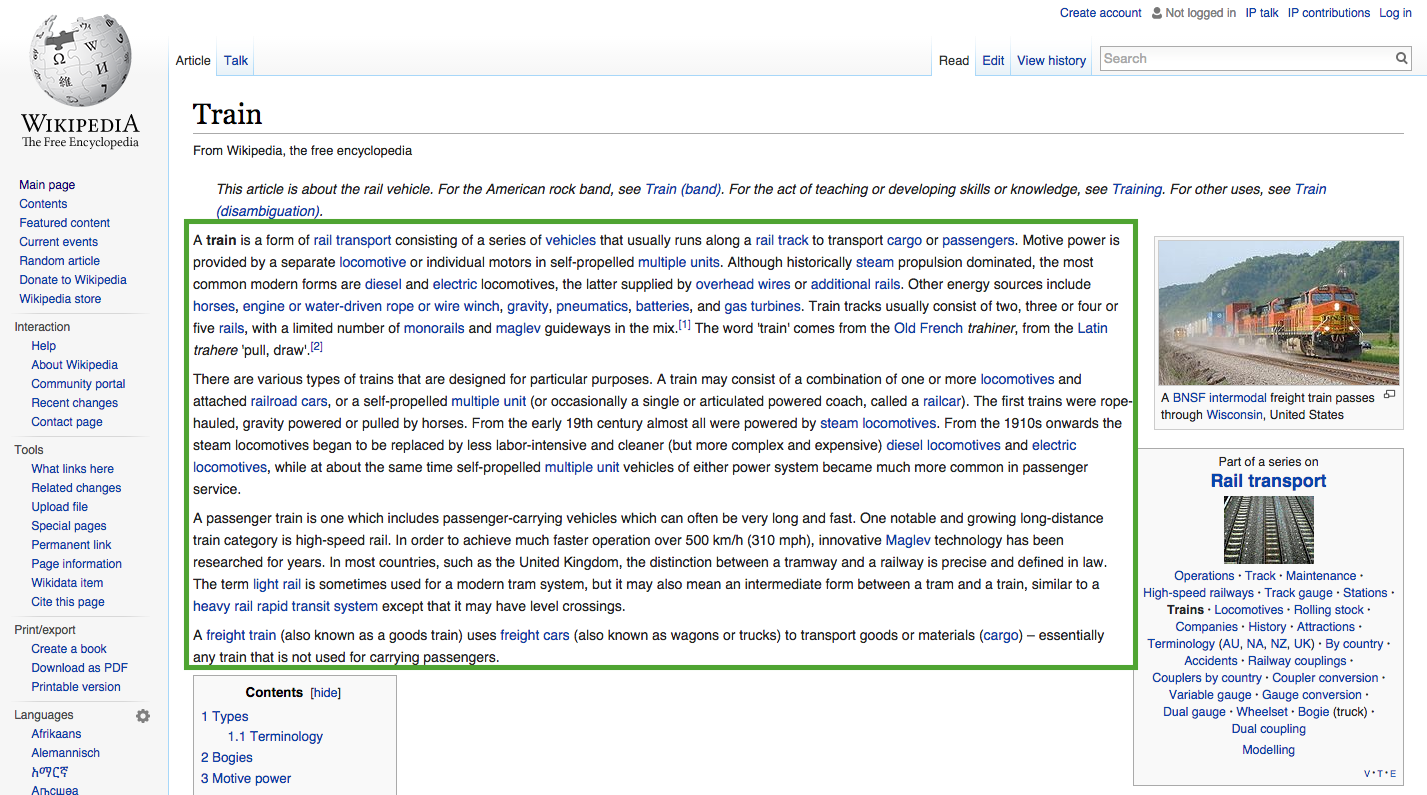
\includegraphics[scale=0.18]{graphics/wiki_train.png}
\ \\

\section{Making a Map: Finding the First Links}
To map Wikipedia's First Link Network, we use the freely-available xml dump of all 4.7 million English articles \cite{2}. We analyze the snapshot provided on November 2014, representing the state of Wikipedia at the time. Knowing Wikipedia is an ever-evolving project with 10 edits every second and 750 new article per day on average \cite{3}, our aim is to characterize the dynamics of the First Link Network, not to record a particular link between one page to another. 

The xml dump provided demarkates article elements in in Media Wiki markup, a markup language with special syntax for links. 
Media Wiki markup also includes templates for audio files, images, side-bar information.
While a human can accurately idenfity the first link, to map the entire First Link Network of 4.7 million pages, we programmatically untangled the body text from side-bar, header box, and bad link elements.

While some libraries exist for Media Wiki Markup, we opted to develop our own algorithm for parsing the first link in the xml version of each article. 
\footnote{Approaches using existing libraries led to several bugs including trouble with nested links, nested parenthesis, unclosed tags, escape characters as well as compatibility with other libraries used to parse the xml.}
Our parsing algorithm aimed to: 1. squash the initial bugs 2. eliminate the need for several passes. To process an article with one pass, we developed a hierachical system of flags:
\begin{itemize}
    \item Flag 1: inside template?
    \begin{itemize}
        \item Flag 2: inside <ref>, <div>?
        \begin{itemize}
            \item Flag 3: inside ()?
        \end{itemize}
    \end{itemize}
\end{itemize}

The algorithm loops in three characters chunks, shifting by one character steps through the article markup. Proceeding in three character chuncks eliminates any nesting issues. If any flag triggers are detected the Flag is raised. Once a flag is raised, we stop processing and proceed to the next character. A first link is correctly identified only if Flags 1, 2, and 3 are all off. Then the entire link is retrieved. We then confirm whether the link is legitimate, meaning it does not link to an image, audio file, external page or other Wikimedia project via keyword triggers provided by Wiki Media \cite{4}. The first link of an article is then the earliest link in the text to pass all three flags and the false link check.


Instead of relying on a sample of articles from which to generalize, we opted to process all 11.blah articles in the xml dump containing the 4.7 million articles along with redirected pages and disambugations, which we filter. To process the entirety of Wikipedia, we divided the xml dump into collections of articles, distributing the processing across 112 cores of the UVM sueprcomputer cluster. We then obtained a complete map of the First Link Network.


\subsection*{testing the algorithm}
\section{Using the Map: Navigating the First Links}

\textcolor{red}{reword the shit below}
\gray{
quote analysis from other areas/dodds paper: Droplets accumulating\\
first paper by Dodds cites Horton-Strahler (leaf pruning) not drop accumulation
}

To understand the structure of Wikipedia's First Link Network, we need to understand how the links flow from one page to another. The procedure, inspired by work in networks/enviromental something ((ask dodds)) is to treat each page as a starting point.

We follow the path of the first links until we reach either a dead link--a page linking to an invalid link (a file, another wikimedia project, or an external webpage)-- or a loop, where one page in the path is revisted.

What we can then measure are various metrics including the number of pages whose path leads to a particular page ((confusing wording)), the path length, even loops of a particular size. Combining these measures, we can then examine are particular properties of how pages related: for example the most popular two-loops.

Thus, from the directed network of First Links, we associate to each node several properties. Fortunately, we need not worry about issues of sampling error or statistiacal accuracy, since we do not rely on any sampling. Instead, thanks to the VACC we are able to follow every single possible path, tallying the properties of each node in the network.

Whether philosophy or another page is at the center of Wikipedia's First Link Network is a question about the page with the most traverses. More importantly, instead of a mere page, we can precisely identify the exact loop structure (or basin) where most pages feed. 

Not only this, we can answer whether the top loop or page is in fact special--whether the number of pages feeding into the page/loop is measurably different from the other top pages/basins.

((add diagram to explain flow of procedure))


\section{The Stories of our Journey: our results}

\subsection{Clicks (beans...)}
Distribution is zipf's law:
((plot))
8.6 million of the 11 million pages in our raw dataset (11 million includes redirects to the subset of 4.2 million actual pages) have no clicks, with less than 1\% of pages accruing more than 100 clicks (precisely 8.56 million of the 11 have no visits).

((maybe sample and graph log-log to see if it's linear to justify zipf's law))

average number of visits is 21.

Even examining only the 1000 pages with the most page visist, we find a majority have no visit:

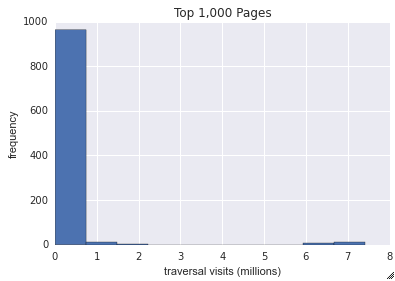
\includegraphics[scale=0.5]{graphics/top_1k_pages.png}

Of the top 100 pages, we see fewer than 30, contain an overwhelming majority of the traversals 6, 7 million:

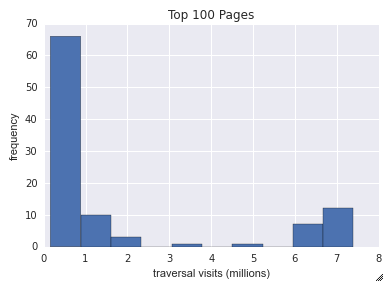
\includegraphics[scale=0.5]{graphics/top_100_pages.png}

Maximum number of traversals is 7.4 million, but the mean is a mere 20 visits. 

The top 7 pages, the ones with teh most visits comprise a loop around philosophy:

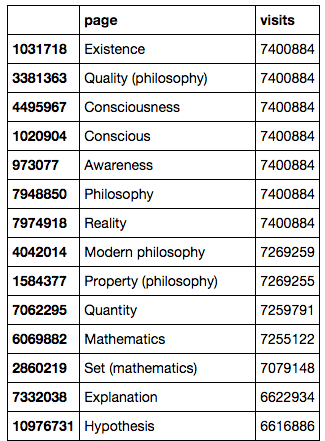
\includegraphics[scale=0.5]{graphics/top_pages_list.png}

\subsection{Longest Path}

The longest first link path span around 365 pages. These paths traverse calendar related pages including religious calendars such as Orthodox Liturgics and history pages. The Eastern Orthodox Liturgics pages for example are dated. Visit any page's Orthodox Liturgics and the first link will send to tomorrow's liturgics. The enxt days links to the following day's liturgics. Curiously, these are complete loops. The last calendar day of the year, simply links back to the first restarting the loop. Other notable pages with a path length of 80 include the legislative assembly of Ontario, 1868 in the UK, 


\subsection{Loops - basics}
Although the loop of 7 pages around philosophy does attract the greatest number of visits, several other loops around natural fundamental concepts also exist. 
The top non-philosophy basins include a basin around community, another around landmass. 

Identifying basins explains the structure of the network, but it doesn't reveal which page/s are a funnel for the basin. By following a similar approach and measuring where the drop accumulation is funneled we find:


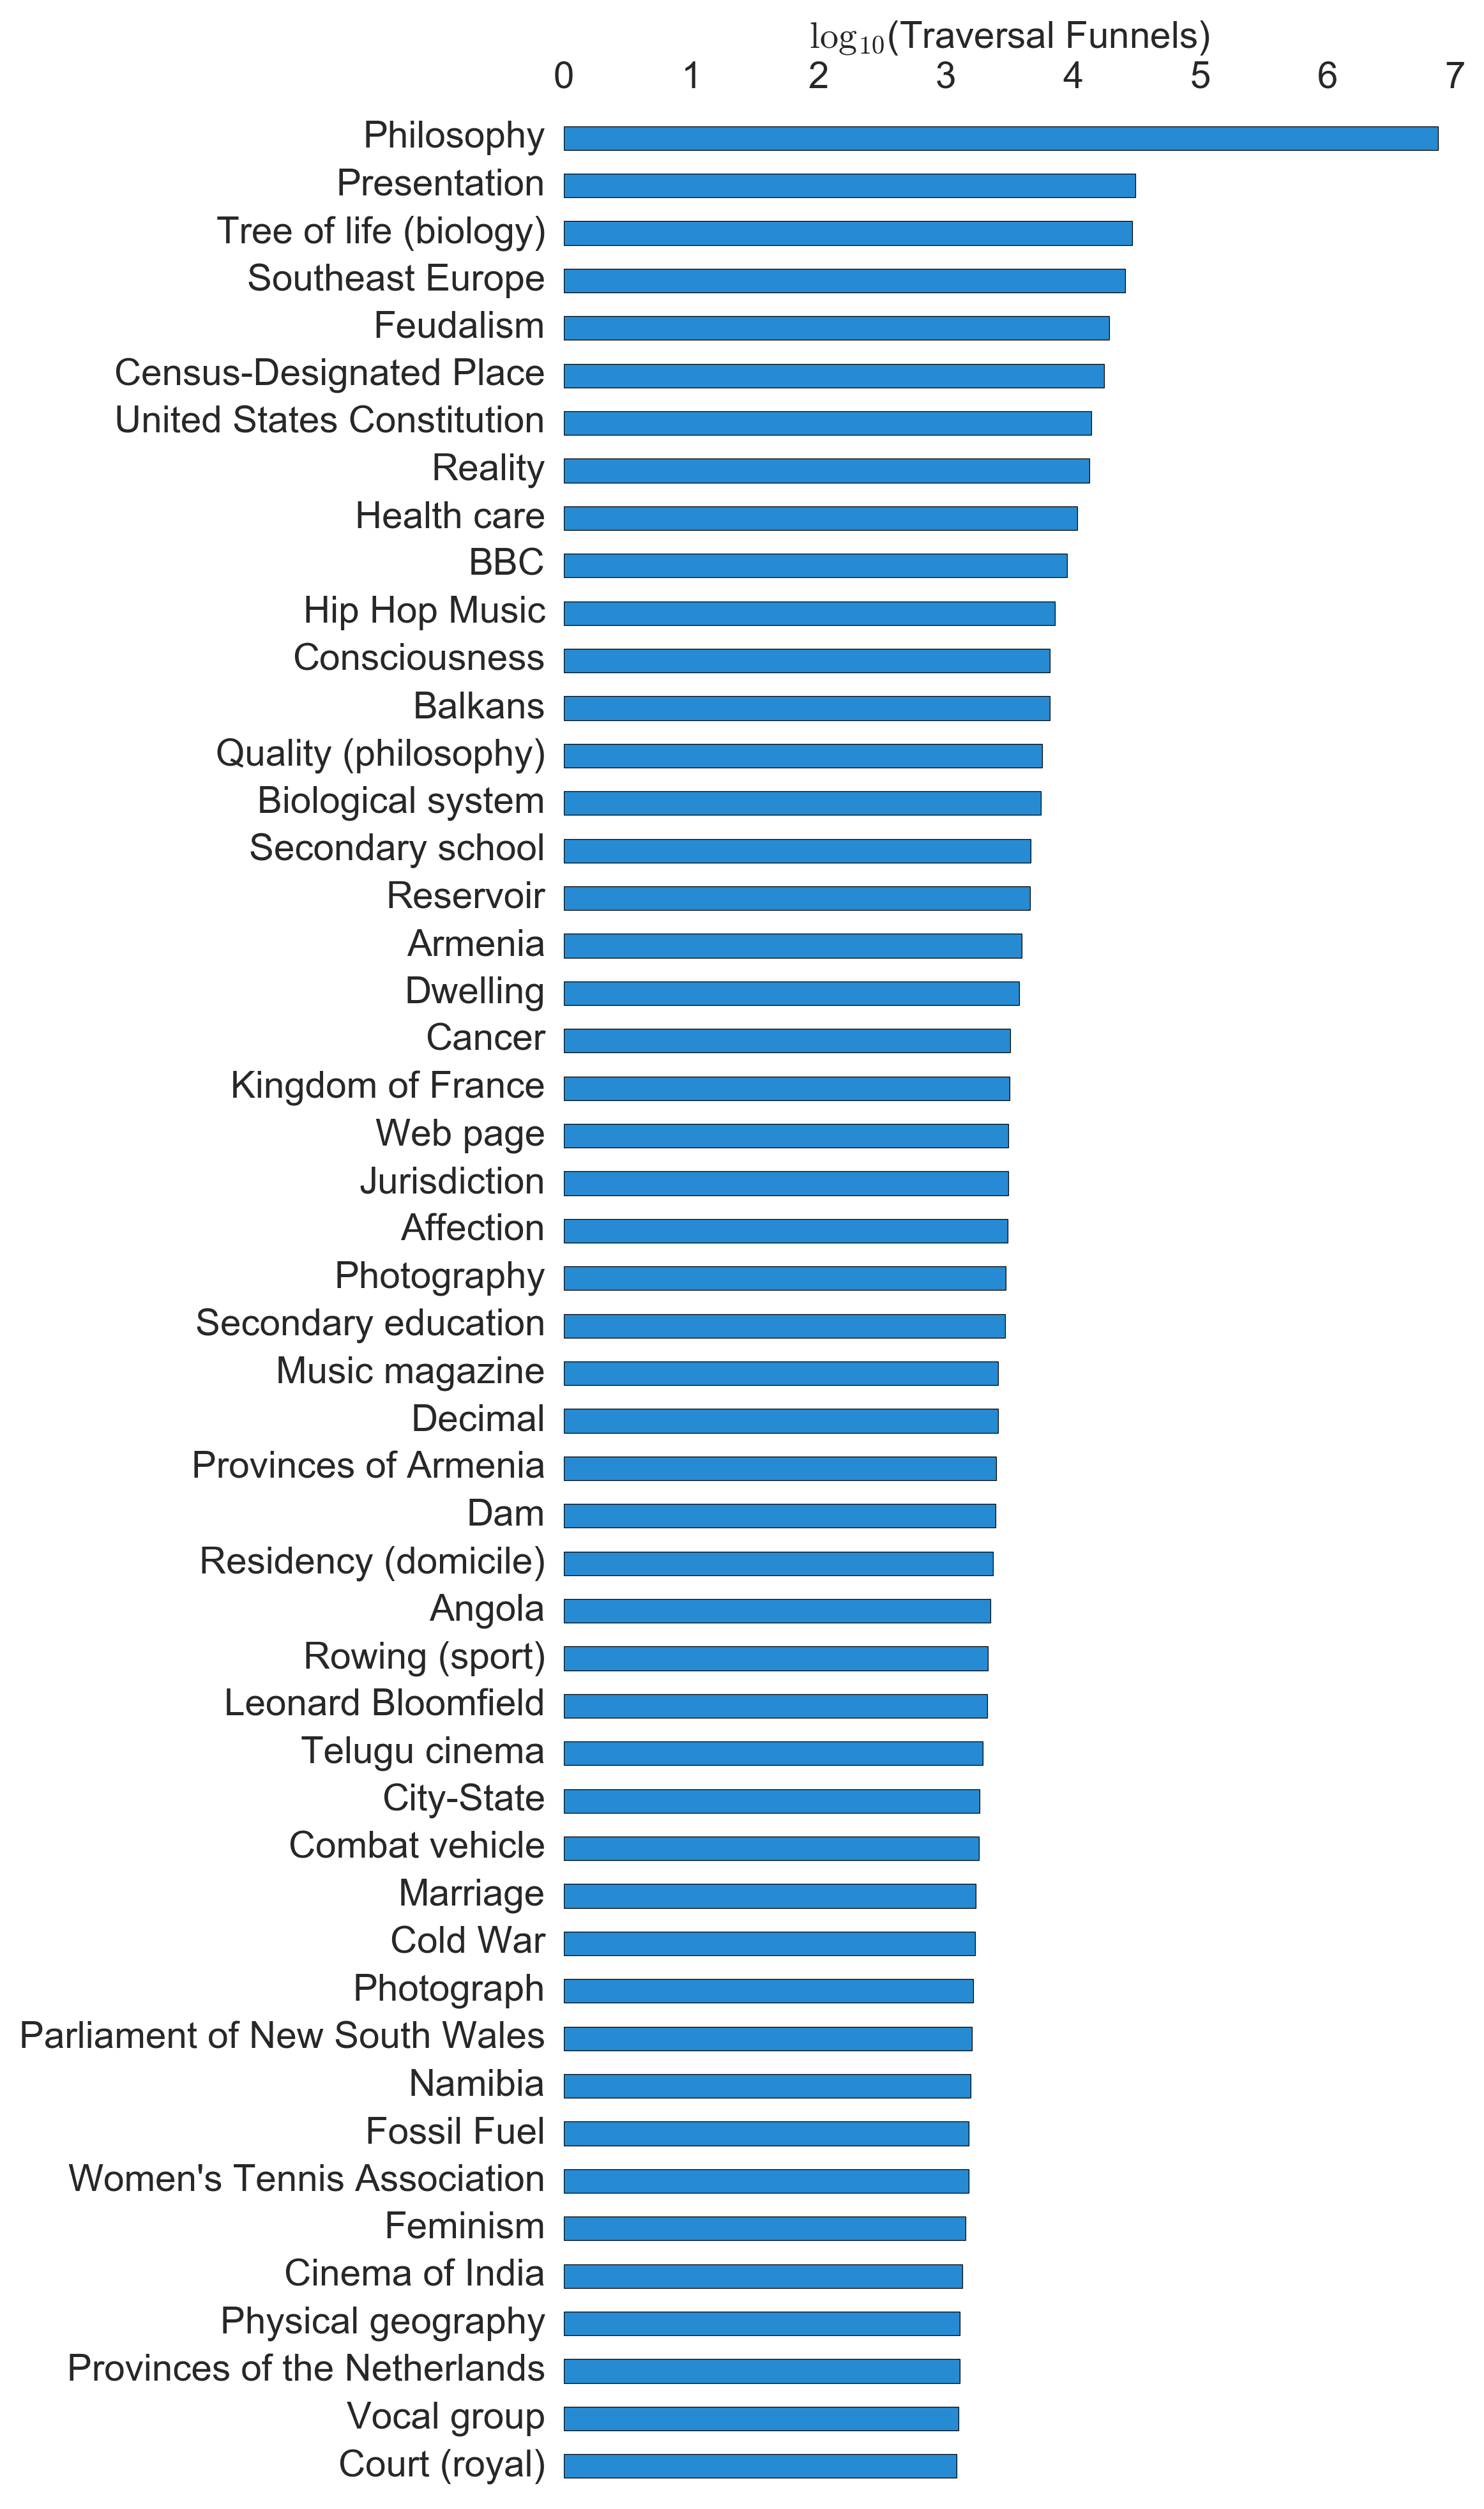
\includegraphics[scale=0.5]{graphics/top_funnels.png}


confirming philosophy is indeed the largest funnel for the philosophy loop, implying it is in fact at the center of wikipedia. Nonetheless, curious foundational funnels also surface such as the word presentation, Tree of life (biology), Geographical regions such as Southern Europe, the US Constituion, health care and BBC. 
This amalgamation mixes both foundational topics, confirming teh theory whereby the first link generalizes a specific page by hooking it to a broader concept. The list also highlights broader topics that are perhaps less foundational, but seem to be at the forefront of people's minds. Health Care while not a foundational discipline such as biology or philosophy ranks at the top perhaps due to the importance we as a society attach to it. Similarly BBC, Hip Hop Music surface perhpas out of a cultural ttraction. 


\red{how many two loops are there compared to the rest of wikipedia?}

In addition to measuring pages that funnel to accumulation, we can also measure true loops instead of just basins. These are pages which sit in a closed loop as opposed ones leading to a dead link.

Furthermore, since we can rank pages, we can rank loops based on the measure associated with each page. We first examine two loops:

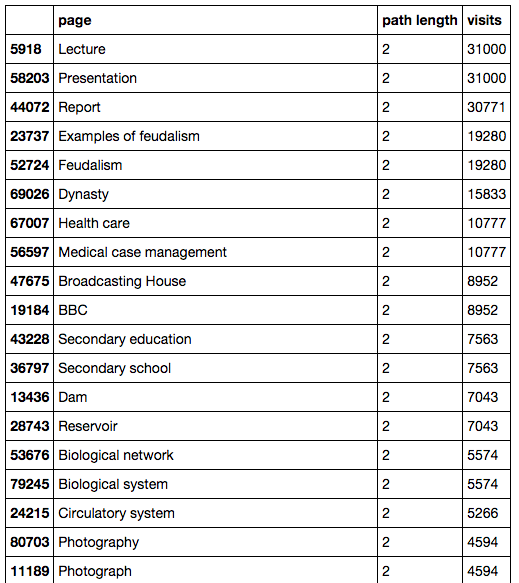
\includegraphics[scale=0.4]{graphics/top_2loops.png}

Two loops reveal ideas that are closely linked to each other or nealry synomous such a secondary school the place wher esecondary education takes place. A lecture which is a form of a presentation, or fedualism and its examples. 

Investigating the list beyond simply the top pages, but looking at a typical 2-loop we find a more natural link between (where typical means between 5 and 15 visits) linking a person to what they are most known for: say a book and author: Anatomy of Britain links to Anthony Sampson (and the reverse; an inventor and their invention: Voere and VEC-91; and an event links to the creator of the event: Peotry Bus Tour links to Wave Books.


While often a less intimate connection, 3-loops reveal a similar pattern. The top ranking 3-loops are:

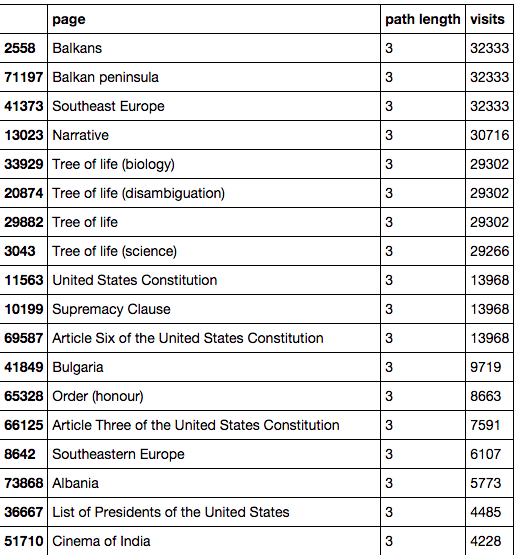
\includegraphics[scale=0.4]{graphics/top_3loops.png}


There are 74k true 3loops.

\subsection{Later: Visualize loops}

\href{http://projects.flowingdata.com/tut/interactive_network_demo/ }{D3 Example 1}

\href{http://christophergandrud.github.io/d3Network/}{simple D3 Network}

\section{Conclusion}

\gray{Next: word stem to see how broader ideas are related (taxonomy of ideas).
    * Broader: what if we consider all links (or first par)? other languages? 
        * popular page by links to it. }

\gray{* Is the network stable over time? 
        * analyze a few newer datasets. }

The analysis remarkably demonstrates the links in Wikipedia truly exihibit a power-law like distribution where most pages link up to a handful of pages. Furthermore, Philosophy does occupy not only a special place inside the most popular basin of attraction. Not only that, the philosophy page itself is the page through which the feeds flow. This implies there is something special even from a mathematical standpoint. Philosophy isn't just a popular link, it lies in an exceptionally high percentage, unique to its loop.

Aside from the philosophy loop, other foundational concepts also emerge as the centers for basins of attraction. Fundamental concepts such as community, government, or philosophy. The network also has a prelevance of 2-loops ((find exact proportion or number)) which link two closely associated concepts such as an inventor or the invention as well as tie synonyms together. Other artifacts such as tremendously long loops based around calendar days demonstrate how we group ideas such as holidays, hisotiric events, or religious, not by their ties to other ideas, but first by where they fall on calendar days. 


Based on the flow from specific pages to more general concepts, the results also agree with the heuristic provided here. Whereby, we link a very specific page to a broader concept, then to an ever broader concept. For example, the Wikipedia page for Banana links to fruit, then botanical then, ((confirm, fill-in)) then biology, then science and eventually philosophy. It is curious that Wikipedia, the largest encyclopedia, which by its very meaning aims to capture information about all branches of human knowledge, has naturally evolved through the works of ((x million editors/edits)) so that Knowledge, philsophy are the center links, occupying such a special place. 


\end{multicols}


\subsection{Terms (aka style guide)}

use article instead of page

traversal = node weight
path length = degree of separation from a cluster
path is the flow from one page until a dead link or a repeated article

cycle (permutation from abstract algebra) instead of loop

basin of attraction or cluster? as opposed to cycle

invalid link (instead of dead or bad link)


To Do:
\textcolor{red}{
\begin{enumerate}
    \item Add limitations of work: snap shot in time, parsing is imperfect
    \item Add better graphics
    \item post code and results to github (add link to paper)
\end{enumerate}}


\newpage

\begin{thebibliography}{10}
\bibitem{1}
\href{ http://www.technologyreview.com/featuredstory/520446/the-decline-of-wikipedia/}{"The Decline of Wikipedia", MIT Tech Review}

\bibitem{2}
\href{https://en.wikipedia.org/wiki/Wikipedia:Database_download}{Wikipedia Database Download}

\bibitem{3}
\href{https://en.wikipedia.org/wiki/Wikipedia:Statistics}{Wikipedia Statistics}

\bibitem{4}
\href{http://en.wikipedia.org/wiki/Help:Special_page}{Media Markup Special Pages}
\end{thebibliography}



\end{document}

